\documentclass[11pt]{article}
\usepackage[utf8]{inputenc}
\usepackage{graphicx}
\usepackage{caption}


\title{Sabina's Emergency Report }
\author{Markovito's team}
%\date[\today]

\begin{document}
\maketitle

% save the image in same folder than tex document
\section{Map of the environment}
This is the mape of the environment where Sabina is looking for somebody.

\begin{figure}
	\begin{center}
		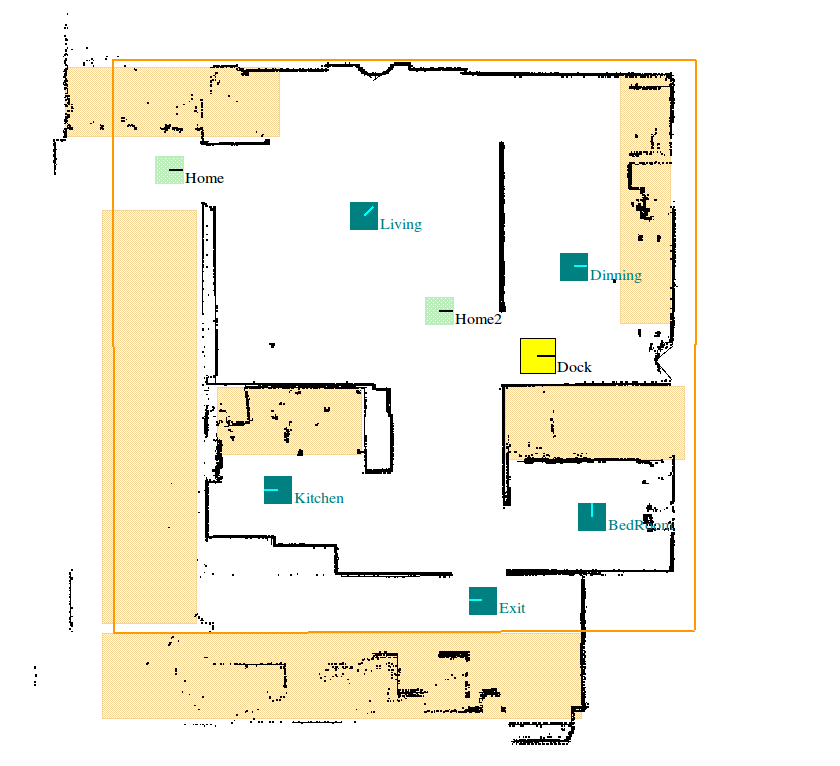
\includegraphics[width=1\textwidth]{map.png}
		\caption{Global Map}
	\end{center}
\end{figure}

\section{Person's location on the map}
The map shows the location where the person was found when he had an accident.

\begin{figure}[h]
	\begin{center}
		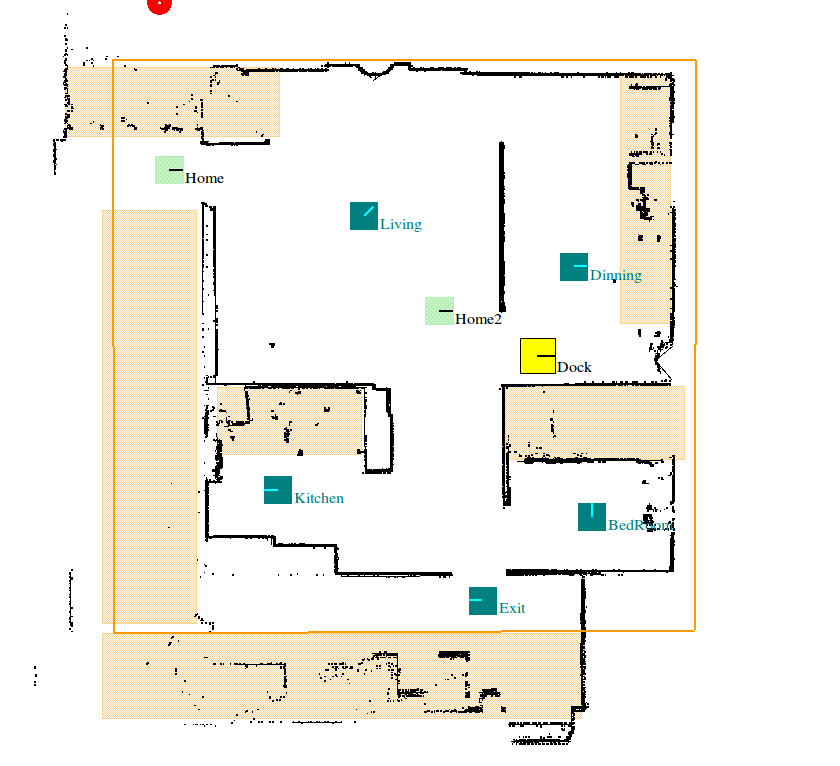
\includegraphics[width=1\textwidth]{locationPeersonHurt.png}
		\caption{The red circle indicates the location of the injured person}
	\end{center}
\end{figure}

\section{Images of the person}

This are the images of the person found.

\begin{figure}[h]
	\begin{center}
		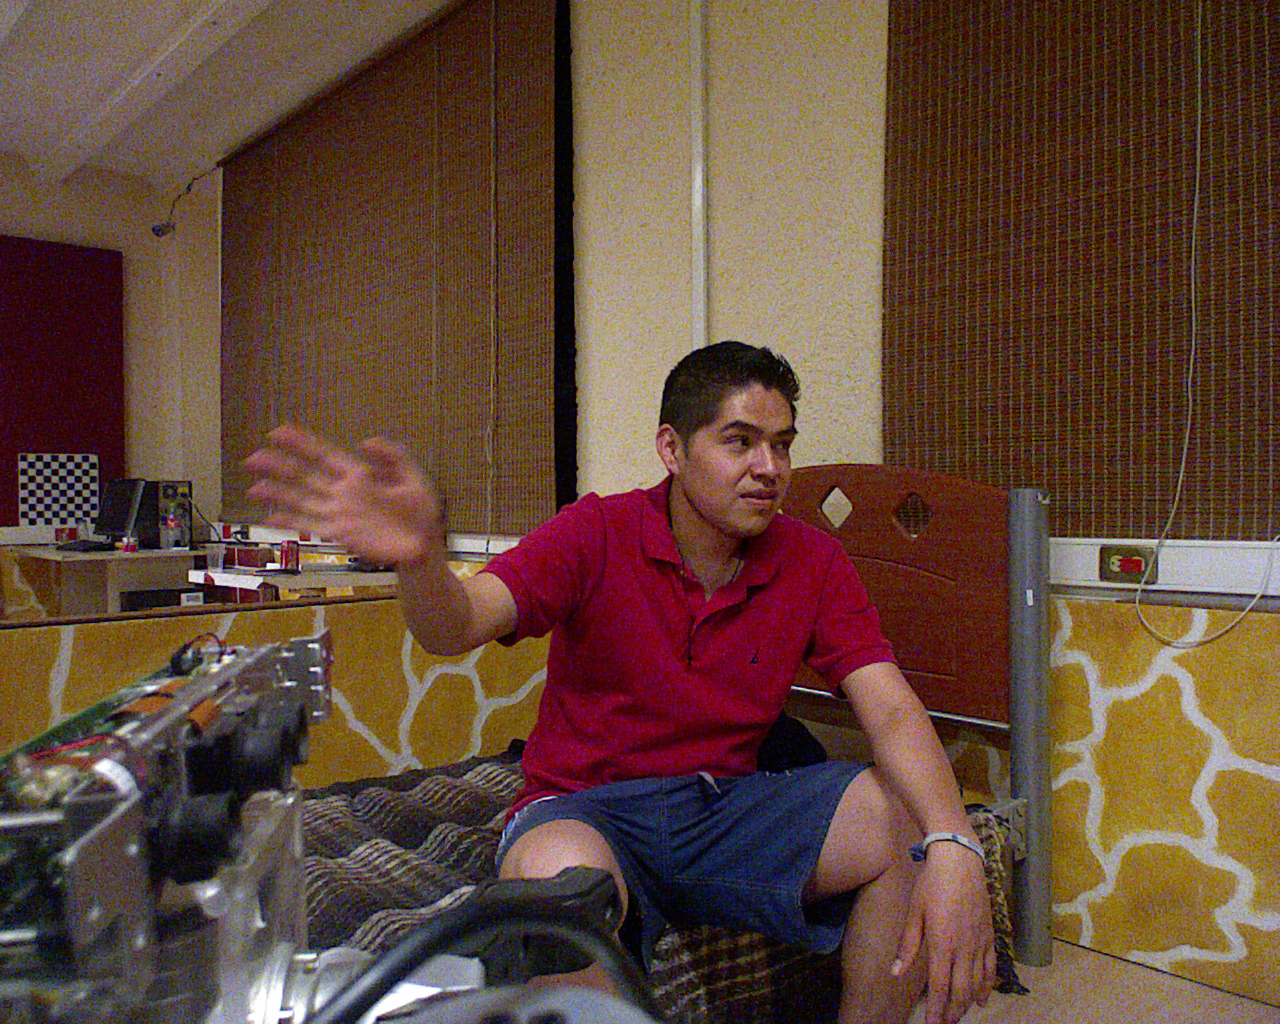
\includegraphics[width=1\textwidth]{imgPeersonHurt.png}
		\caption{This is an image showing the persons condition}
	\end{center}
\end{figure}

\section{Object requested}

Object requested by person.

\begin{figure}[h]
	\begin{center}
		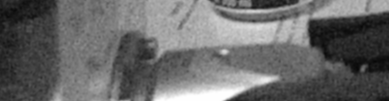
\includegraphics[width=1\textwidth]{EmergencyObjectRequested.png}
		\caption{the injured person requested me to bring him this object}
	\end{center}
\end{figure}



\end{document}
